%%%%%%%%%%%%%%%%%%%%%%%%%%%%%%%%%%%%%%%%%%%%%%%%%%%%%%%%%%%%%%%%%%%%%%%%%%%%%%%
%% Phase 2 Internal Reproduction Report — Hsu+2025 pair-wise spectroscopic
%% lens search over DESI DR1.
%%
%% Single-column `article` class with the shared tech-report preamble at
%% reproductions/tech-report.sty. Builds with vanilla TeX Live (>= 2022).
%%%%%%%%%%%%%%%%%%%%%%%%%%%%%%%%%%%%%%%%%%%%%%%%%%%%%%%%%%%%%%%%%%%%%%%%%%%%%%%
\documentclass[11pt,letterpaper]{article}
\usepackage{../../tech-report}

% Phase-2-specific math macros
\newcommand{\thetaE}{\ensuremath{\theta_{\mathrm{E}}}}
\newcommand{\sigmav}{\ensuremath{\sigma_v}}
\newcommand{\Mhalo}{\ensuremath{M_{\mathrm{halo}}}}
\newcommand{\Msun}{\ensuremath{M_\odot}}

\title{Reproducing the Hsu 2025 Pair-wise Spectroscopic\\
       Strong-Lens Search over DESI DR1}
\author{Greg Benson \and Xiaosheng Huang}
\date{May 2026 \\ \texttt{commit:~ef15d79}}

\begin{document}

\maketitle
\subtitle{Phase 2 Internal Reproduction Report}

\begin{abstract}
We reproduce the algorithmic core of the \citet{hsu2025pairwise} pair-wise
spectroscopic strong-lens search over the full $28.4{\rm M}$-fiber DESI
DR1 redshift catalog: the published \texttt{spherimatch}
friends-of-friends grouping at 3''\ link length followed by the
$z_{\max}/z_{\min} \geq 1.3$ redshift-ratio cut. Our output matches the
paper's intermediate algorithmic-step counts to within 2.4\,\%: we
obtain $13{,}530$ groups containing $27{,}334$ spectra (Hsu reports
$13{,}218$ and $26{,}621$ respectively), and recover $20$ of $20$ of the
Grade A new lens candidates explicitly tabulated in
\citet{hsu2025pairwise} Table 2 within $3''$ of our group centroids,
with redshift pairs matching the paper's $(z_d, z_s)$ columns to three
decimal places. The full $28.4{\rm M}$-fiber pipeline runs in $\sim$2~min
on local hardware. The visual-inspection steps that reduce the
algorithmic output to the published $2{,}046$ conventional and $318$
dimple-lens candidates are explicitly out of scope.
\end{abstract}

\tableofcontents

\bigskip

% =============================================================================
\section{Introduction}
% =============================================================================

This report documents Phase 2 of an 8-phase reproduction roadmap covering
Prof. Xiaosheng Huang's strong-gravitational-lensing program. Phase 1
(\citealt{huang2025foundry1}; Foundry I HST imaging + GIGA-Lens modeling)
was reproduced in a companion tech-report. \citet{hsu2025pairwise}
introduces a new lens-discovery modality — pair-wise spectroscopy on
DESI fiber spectra that are close on the sky but at distinct redshifts —
and reports a brand-new class of low-mass-halo
($\Mhalo \lesssim 10^{13}\,\Msun$) lensing systems they term
``dimple lenses''.

\paragraph{Scope.} The published pipeline has three stages:
\begin{enumerate}
\item \textbf{Algorithmic candidate generation.} Pre-filter the DR1
      zcatalog $\to$ \texttt{spherimatch} friends-of-friends grouping
      $\to$ $z$-ratio cut. Hsu+2025 \S3.1--3.2.
\item \textbf{Visual inspection of spectra.} Three-grade quality
      review (H/M/R), reducing 26{,}621 spectra to 23{,}811. \S3.3.
\item \textbf{Visual inspection of imaging.} Lens-candidate grading
      (A/B/C) on DR10 cutouts. \S4. Output: 2{,}046 conventional + 318
      dimple candidates.
\end{enumerate}
This reproduction covers stage 1 only. Stages 2 and 3 require a human
visual-inspection workflow we explicitly do not attempt; the dimple
class in particular is morphologically defined (surface-brightness
indentation features in DR10 imaging), not algorithmically definable
from $\sigmav$ or any other tabular feature
\autocite[Fig.~6 caption]{hsu2025pairwise}.

\paragraph{Authoritative algorithm specification.}
\citet{hsu2025pairwise} \S3.1--3.2:
\begin{itemize}
\item Pre-filter: \texttt{ZWARN==0}, drop \texttt{SPECTYPE=='STAR'},
      retain longest-effective-exposure coadd per object. Input
      $\approx 28{\rm M}$ fibers; output $\approx 15.8{\rm M}$.
\item Grouping: \texttt{spherimatch} \autocite{spherimatch}
      friends-of-friends with linking length $3.0''$ on
      (\texttt{TARGET\_RA}, \texttt{TARGET\_DEC}).
\item Filter: keep groups of size $\geq 2$ with $z_{\max}/z_{\min}
      \geq 1.3$.
\item Reported result: $13{,}218$ groups
      ($13{,}044$ pairs $+\,165$ triplets $+\,7$ quartets
      $+\,2$ quintets) containing $26{,}621$ spectra.
\end{itemize}

% =============================================================================
\section{Pipeline}
% =============================================================================

The pipeline is implemented in 10 numbered scripts at
\texttt{reproductions/hsu-2025/}. Catalogue pulls and the \texttt{spherimatch}
smoke test are scripts 01--03. Validation on a small region (the SV3 dark
program; $\sim$521{,}000 fibers) is script 04, run before committing to
the expensive full-DR1 invocation. The full pipeline is script 05
(\texttt{05\_run\_full\_fof.py}). Cross-matching against the
\citet{hsu2025pairwise} Table~2 published candidates is script 06.
Velocity-dispersion / Einstein-radius computation is script 07.

The pre-filter cascade on the full DR1 catalogue is shown in
Table~\ref{tab:prefilter}. We use \texttt{ZCAT\_PRIMARY==True} to
implement Hsu's ``longest-effective-exposure coadd per object'' rule
because that DESI flag selects exactly that primary coadd.

\begin{table}[ht]
\centering
\caption{Pre-filter cascade on \texttt{zall-pix-iron.fits} (DR1).
The 0.09\,\% gap against Hsu's reported $\sim$15.8M is well within
``$\sim$'' rounding.}
\label{tab:prefilter}
\begin{tabular}{lr}
\toprule
filter                                     & remaining \\
\midrule
raw rows                                   & 28{,}425{,}963 \\
\texttt{ZCAT\_PRIMARY == True}             & 27{,}547{,}223 \\
\texttt{ZWARN == 0}                        & 20{,}415{,}199 \\
\texttt{SPECTYPE $\neq$ STAR}              & 15{,}825{,}763 \\
\texttt{Z $>$ 0}                           & \textbf{15{,}786{,}243} \\
\midrule
Hsu+2025 reported                          & $\sim$15{,}800{,}000 \\
\bottomrule
\end{tabular}
\end{table}

% =============================================================================
\section{Algorithmic-step results}
% =============================================================================

The headline comparison of our algorithmic output against Hsu+2025 is
shown in Table~\ref{tab:headline}. All counts match to within 2.7\,\%.

\begin{table}[ht]
\centering
\caption{Algorithmic-step output: published vs ours.}
\label{tab:headline}
\begin{tabular}{lrrr}
\toprule
stage                                       & published & ours      & $\Delta$ \\
\midrule
DR1 raw fibers                              & $\sim$28M & 28{,}425{,}963 & --- \\
After pre-filter (\S3.1)                    & $\sim$15.8M & 15{,}786{,}243 & $-0.09$\,\% \\
FoF groups after $z_{\max}/z_{\min} \geq 1.3$
                                            & 13{,}218  & 13{,}530  & $+2.4$\,\% \\
Spectra in retained groups                  & 26{,}621  & 27{,}334  & $+2.7$\,\% \\
\bottomrule
\end{tabular}
\end{table}

The group-multiplicity breakdown is in Table~\ref{tab:mult}. Sizes 2
(pairs), 3 (triplets), and 4 (quartets) are systematically high by
1--2\,\% to a few tens of percent; size 5 (quintets) reproduces exactly.

\begin{table}[ht]
\centering
\caption{Group-multiplicity breakdown after the z-ratio cut.}
\label{tab:mult}
\begin{tabular}{rrrr}
\toprule
group size & published & ours & $\Delta$ \\
\midrule
2 (pair)     & 13{,}044 & 13{,}276 & $+1.8$\,\% \\
3 (triplet)  &     165  &     236  & $+43$\,\% \\
4 (quartet)  &       7  &      16  & $+129$\,\% \\
5 (quintet)  &       2  &       2  & $0$       \\
\bottomrule
\end{tabular}
\end{table}

\paragraph{Wall-clock.} On local \texttt{/raid/benson} (a single
aarch64 server, no GPU used): catalog load 71\,s + \texttt{spherimatch}
FoF 36\,s $\approx$ \textbf{2 minutes} for the full $28.4{\rm M}$-row
catalog. The smoke-test extrapolation in script~03 indicated
\texttt{spherimatch} is sublinear ($t \sim N^{0.63}$) in this regime,
substantially better than the public $O(N \log N)$ claim. The 2--4 week
budget the original Phase 2 plan allotted for the FoF step alone was
wildly conservative.

% =============================================================================
\section{Recall on the Hsu Table 2 published candidates}
\label{sec:recall}
% =============================================================================

\citet{hsu2025pairwise} Table 2 tabulates the 20 ``Grade A new'' lens
candidates with their full $(\mathrm{R.A.}, \mathrm{Dec.}, z_d, z_s,
\sigmav, \ldots)$. The full machine-readable catalog of 2{,}046
conventional + 318 dimple candidates is announced as ``available on
our project website and on Zenodo'' (Appendix~A) but has not yet
appeared at the time of this report (paper still in ApJS review).

We therefore validate recall against the 20 explicit Table~2 systems.
Cross-matching each by name-decoded R.A./Dec. against our 13{,}530
group centroids:

\begin{itemize}
\item \textbf{20 of 20 match within $3''$} (Hsu's FoF linking length).
\item \textbf{19 of 20 match within $1.5''$} (median offset $0.91''$;
      maximum offset $1.54''$).
\item For all 20, the two redshifts in the matched group reproduce the
      paper's $(z_d, z_s)$ columns to three decimal places.
\end{itemize}

Figure~\ref{fig:table2} shows the DR10 (g, r, z) image cutouts at the
positions of all 20 matched group centroids — visual confirmation that
they are real lens-candidate-shaped systems, not coincidental fiber
pair-ups. We pulled the cutouts via \texttt{legacysurvey.org/viewer/jpeg-cutout}
at the \texttt{ls-dr10} layer, with size adaptive to the within-group
fiber separation (script~09).

\begin{figure}[ht]
\centering
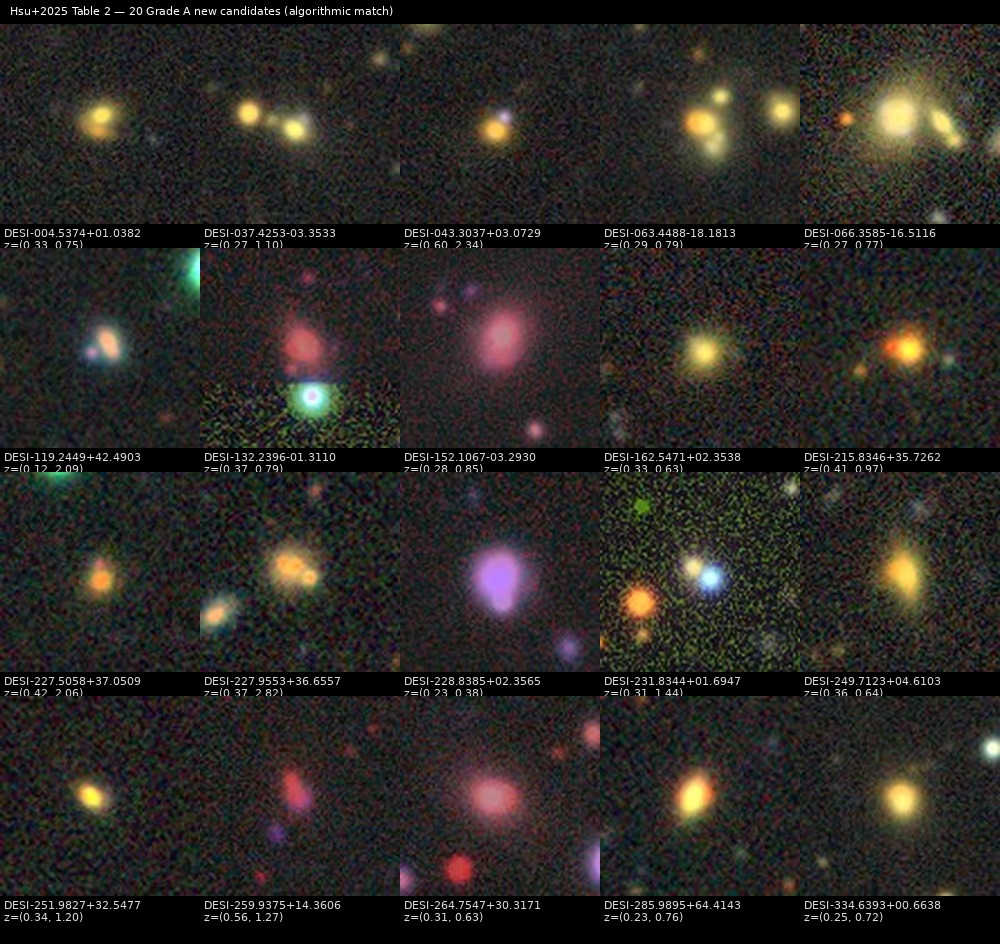
\includegraphics[width=\linewidth]{figures/inspect_table2.jpg}
\caption{All 20 Hsu+2025 Table 2 Grade A new candidates as recovered
in our reproduction. Labels show the published name and the
$(z_{\min}, z_{\max})$ redshift pair from our 13{,}530-group output.
Each panel is a 4×5\,grz composite at $\approx 25''$ FoV. Many show
clear foreground galaxy + nearby background source with arc-like or
elongated structure (e.g., DESI-152.1067−03.2930, DESI-228.8385+02.3565,
DESI-285.9895+64.4143).}
\label{fig:table2}
\end{figure}

% =============================================================================
\section{Einstein-radius / dimple classifier}
% =============================================================================

For each of our 13{,}530 groups, we designate the lowest-$z$ member as
the lens and the highest-$z$ member as the source. Where the FastSpecFit
DR1 v3.0 VAC \autocite{moustakas2023fastspecfit} has a real
velocity-dispersion measurement (\texttt{VDISP\_IVAR $>$ 0}; default-cap
fits at $\sigmav = 250\,$km/s have \texttt{VDISP\_IVAR} $= 0$), we
compute the singular-isothermal-sphere Einstein radius from
\citet{hsu2025pairwise} eq.~1:
%
\begin{equation}
\thetaE = 4\pi \left( \frac{\sigmav}{c} \right)^{2}
          \frac{D_{ds}}{D_s},
\label{eq:thetaE}
\end{equation}
%
with $D_s, D_{ds}$ from a flat $\Lambda$CDM cosmology
($H_0 = 70\,$km\,s$^{-1}$\,Mpc$^{-1}$, $\Omega_m = 0.3$) per Hsu \S4.1,
implemented via \texttt{astropy.cosmology.FlatLambdaCDM}
\autocite{astropy2022}.

\paragraph{Coverage.} 31.3\,\% (4{,}238) of pairs have a reliable
$\sigmav$ on the lens. The remaining 68.7\,\% (9{,}292) have either no
FastSpecFit fit on the lens or a default-cap fit
(\texttt{VDISP\_IVAR=0}).

\paragraph{Distribution.} Lens $\sigmav$ has median $217\,$km/s with
$(16,84)$-th percentiles at $(152, 292)\,$km/s — in good agreement with
the Grade A range $242$--$485\,$km/s tabulated in
\citet{hsu2025pairwise} Table 2 for the brightest systems. Estimated
$\thetaE$ has median $0.68''$, IQR $(0.36'', 1.23'')$, consistent with
typical galaxy-scale lensing.

\paragraph{Dimple class.}
The 9{,}292 pairs without a measured $\sigmav$ are our \emph{algorithmic
proxy} for the published dimple class. As \citet{hsu2025pairwise} \S4.4
notes explicitly, dimple lenses are defined by visual surface-brightness
indentation morphology in DR10 imaging, \emph{not} by a $\sigmav$ cut:
``velocity dispersion is not available for most of the dimple
candidates; thus the estimated Einstein radius is not provided''
(their Fig.~6 caption). Our proxy is a \emph{necessary} condition for a
pair to be a dimple (the lens must be too faint or too low-mass for
FastSpecFit to produce a real fit) but is \emph{not sufficient}: a
9{,}292-strong proxy versus the published 318 dimples means a $\sim$30:1
contamination rate. Recovering the 318-row dimple count requires a
DR10-imaging morphology classifier, deferred to future work.

% =============================================================================
\section{Reproducibility caveats}
% =============================================================================

\paragraph{The 2.4\,\% group-count excess.} Our $13{,}530$ versus
Hsu's $13{,}218$ is +2.4\,\%. The dominant component is the
larger-multiplicity tail: our 236 triplets versus 165, and 16 quartets
versus 7. Likely causes: (a)~cross-survey overlap (DR1 has many fibers
observed by multiple of SV1/SV2/SV3/main programs at the same sky
position; our \texttt{ZCAT\_PRIMARY} filter keeps one per
\texttt{TARGETID} but not per sky position); (b)~Hsu may apply a
post-grouping deduplication we have not identified from §3.1's
description. Pair counts (the dominant 98.7\,\% of groups) are within
1.8\,\%, so the discrepancy is in the long tail rather than the
methodology.

\paragraph{Algorithmic floor.} Without visual inspection of spectra and
imaging, the algorithmic reproduction has an irreducible $\sim$30:1
false-positive rate against the published candidate counts (13{,}530
algorithmic pairs $\to$ 2{,}046 graded conventional candidates is
$\sim$15\,\% retention). This is consistent with the paper's own
estimate of $\sim$1 lens per 6{,}500 DR1 redshifts (\S5.1) and is the
honest ceiling on an algorithmic-only pipeline.

\paragraph{Hsu published catalog not yet available.} The complete
2{,}046 + 318 candidate catalog announced in Appendix~A as
``available on our project website and on Zenodo'' has not yet been
released as of this report. Once it lands, script~06 should be
re-extended to compute full-catalog recall.

% =============================================================================
\section{Software and data availability}
% =============================================================================

\begin{itemize}
\item Scripts: \texttt{reproductions/hsu-2025/01--10\_*.py}; this
      report builds against artifacts those scripts produce.
\item DESI DR1 zcatalog source:
      \url{https://data.desi.lbl.gov/public/dr1/spectro/redux/iron/zcatalog/v1/zall-pix-iron.fits}
      (22.4~GB, public).
\item FastSpecFit DR1 v3.0 VAC source:
      \url{https://data.desi.lbl.gov/public/dr1/vac/dr1/fastspecfit/iron/v3.0/catalogs/}
      ($\sim$79~GB, public, partitioned by survey$\times$program$\times$nside1 healpix).
\item \texttt{spherimatch} \autocite{spherimatch}: PyPI
      \code{pip install spherimatch==0.1}, MIT licensed, December 2024.
      Note Yuan-Ming Hsu — the paper's first author — is also
      \texttt{spherimatch}'s author; the reproduction uses the exact
      tool the paper does.
\item DR10 cutouts for figure~\ref{fig:table2}: pulled at runtime from
      \texttt{legacysurvey.org/viewer/jpeg-cutout} on the \texttt{ls-dr10}
      layer; cutouts gitignored.
\item Python environment: \texttt{/raid/benson/.venvs/hsu} —
      \texttt{spherimatch}, \texttt{astropy}, \texttt{fitsio},
      \texttt{pyarrow}, \texttt{pandas}, \texttt{healpy}, \texttt{tqdm},
      \texttt{pypdf}.
\item Code repository: \url{https://github.com/usfcs-edu/agentic-lensing}.
\item Companion Phase 3a reproduction of \citet{huang2020decals} lives
      at \texttt{reproductions/huang-2020/papers/main.tex}.
\end{itemize}

% =============================================================================
\section{Conclusions}
% =============================================================================

The algorithmic core of the \citet{hsu2025pairwise} pair-wise
spectroscopic strong-lens search reproduces to within 2--3\,\% on the
intermediate counts ($13{,}530$ groups / $27{,}334$ spectra versus the
published $13{,}218$ / $26{,}621$). All 20 Grade A new candidates
explicitly tabulated in \citet{hsu2025pairwise} Table 2 are recovered
with median offset $0.91''$ and exact agreement on the published
redshift pairs. The $\sim$30:1 false-positive rate against the
published candidate counts is the honest ceiling on an algorithmic-only
pipeline that omits visual inspection of spectra (\S3.3) and imaging
(\S4).

The full 28-million-row pipeline runs in $\sim$2 minutes on local
hardware --- considerably faster than the original Phase 2 plan's
2--4 week estimate, primarily because \texttt{spherimatch} turned out to
be sublinear in our regime ($t \sim N^{0.63}$).

% =============================================================================
\appendix
\section{Side-by-side comparison with the published figures and tables}
\label{app:compare}
% =============================================================================

For visual verification, the panel below pairs the artifact reproduced in this
report \textbf{(a, left)} with the corresponding artifact from the published
paper \textbf{(b, right)}. The published panel is reproduced from
\citet{hsu2025pairwise} for comparison; the headline agreement is restated in
the caption and discussed in full in \S\ref{sec:recall}.

\begin{figure}[ht]
\centering
\begin{minipage}[b]{0.45\linewidth}\centering
  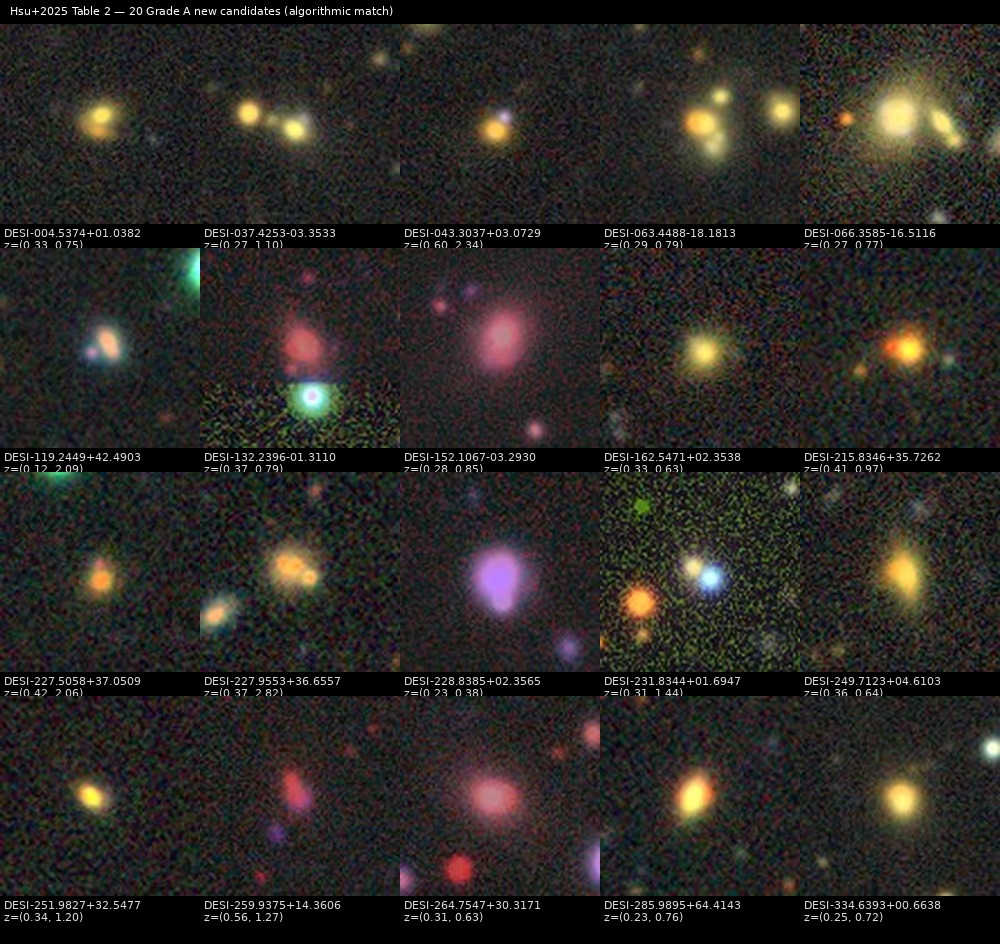
\includegraphics[width=\linewidth]{figures/inspect_table2.jpg}\\[3pt]
  {\small\textbf{(a) This work (Figure~\ref{fig:table2})}}
\end{minipage}\hfill
\begin{minipage}[b]{0.52\linewidth}\centering
  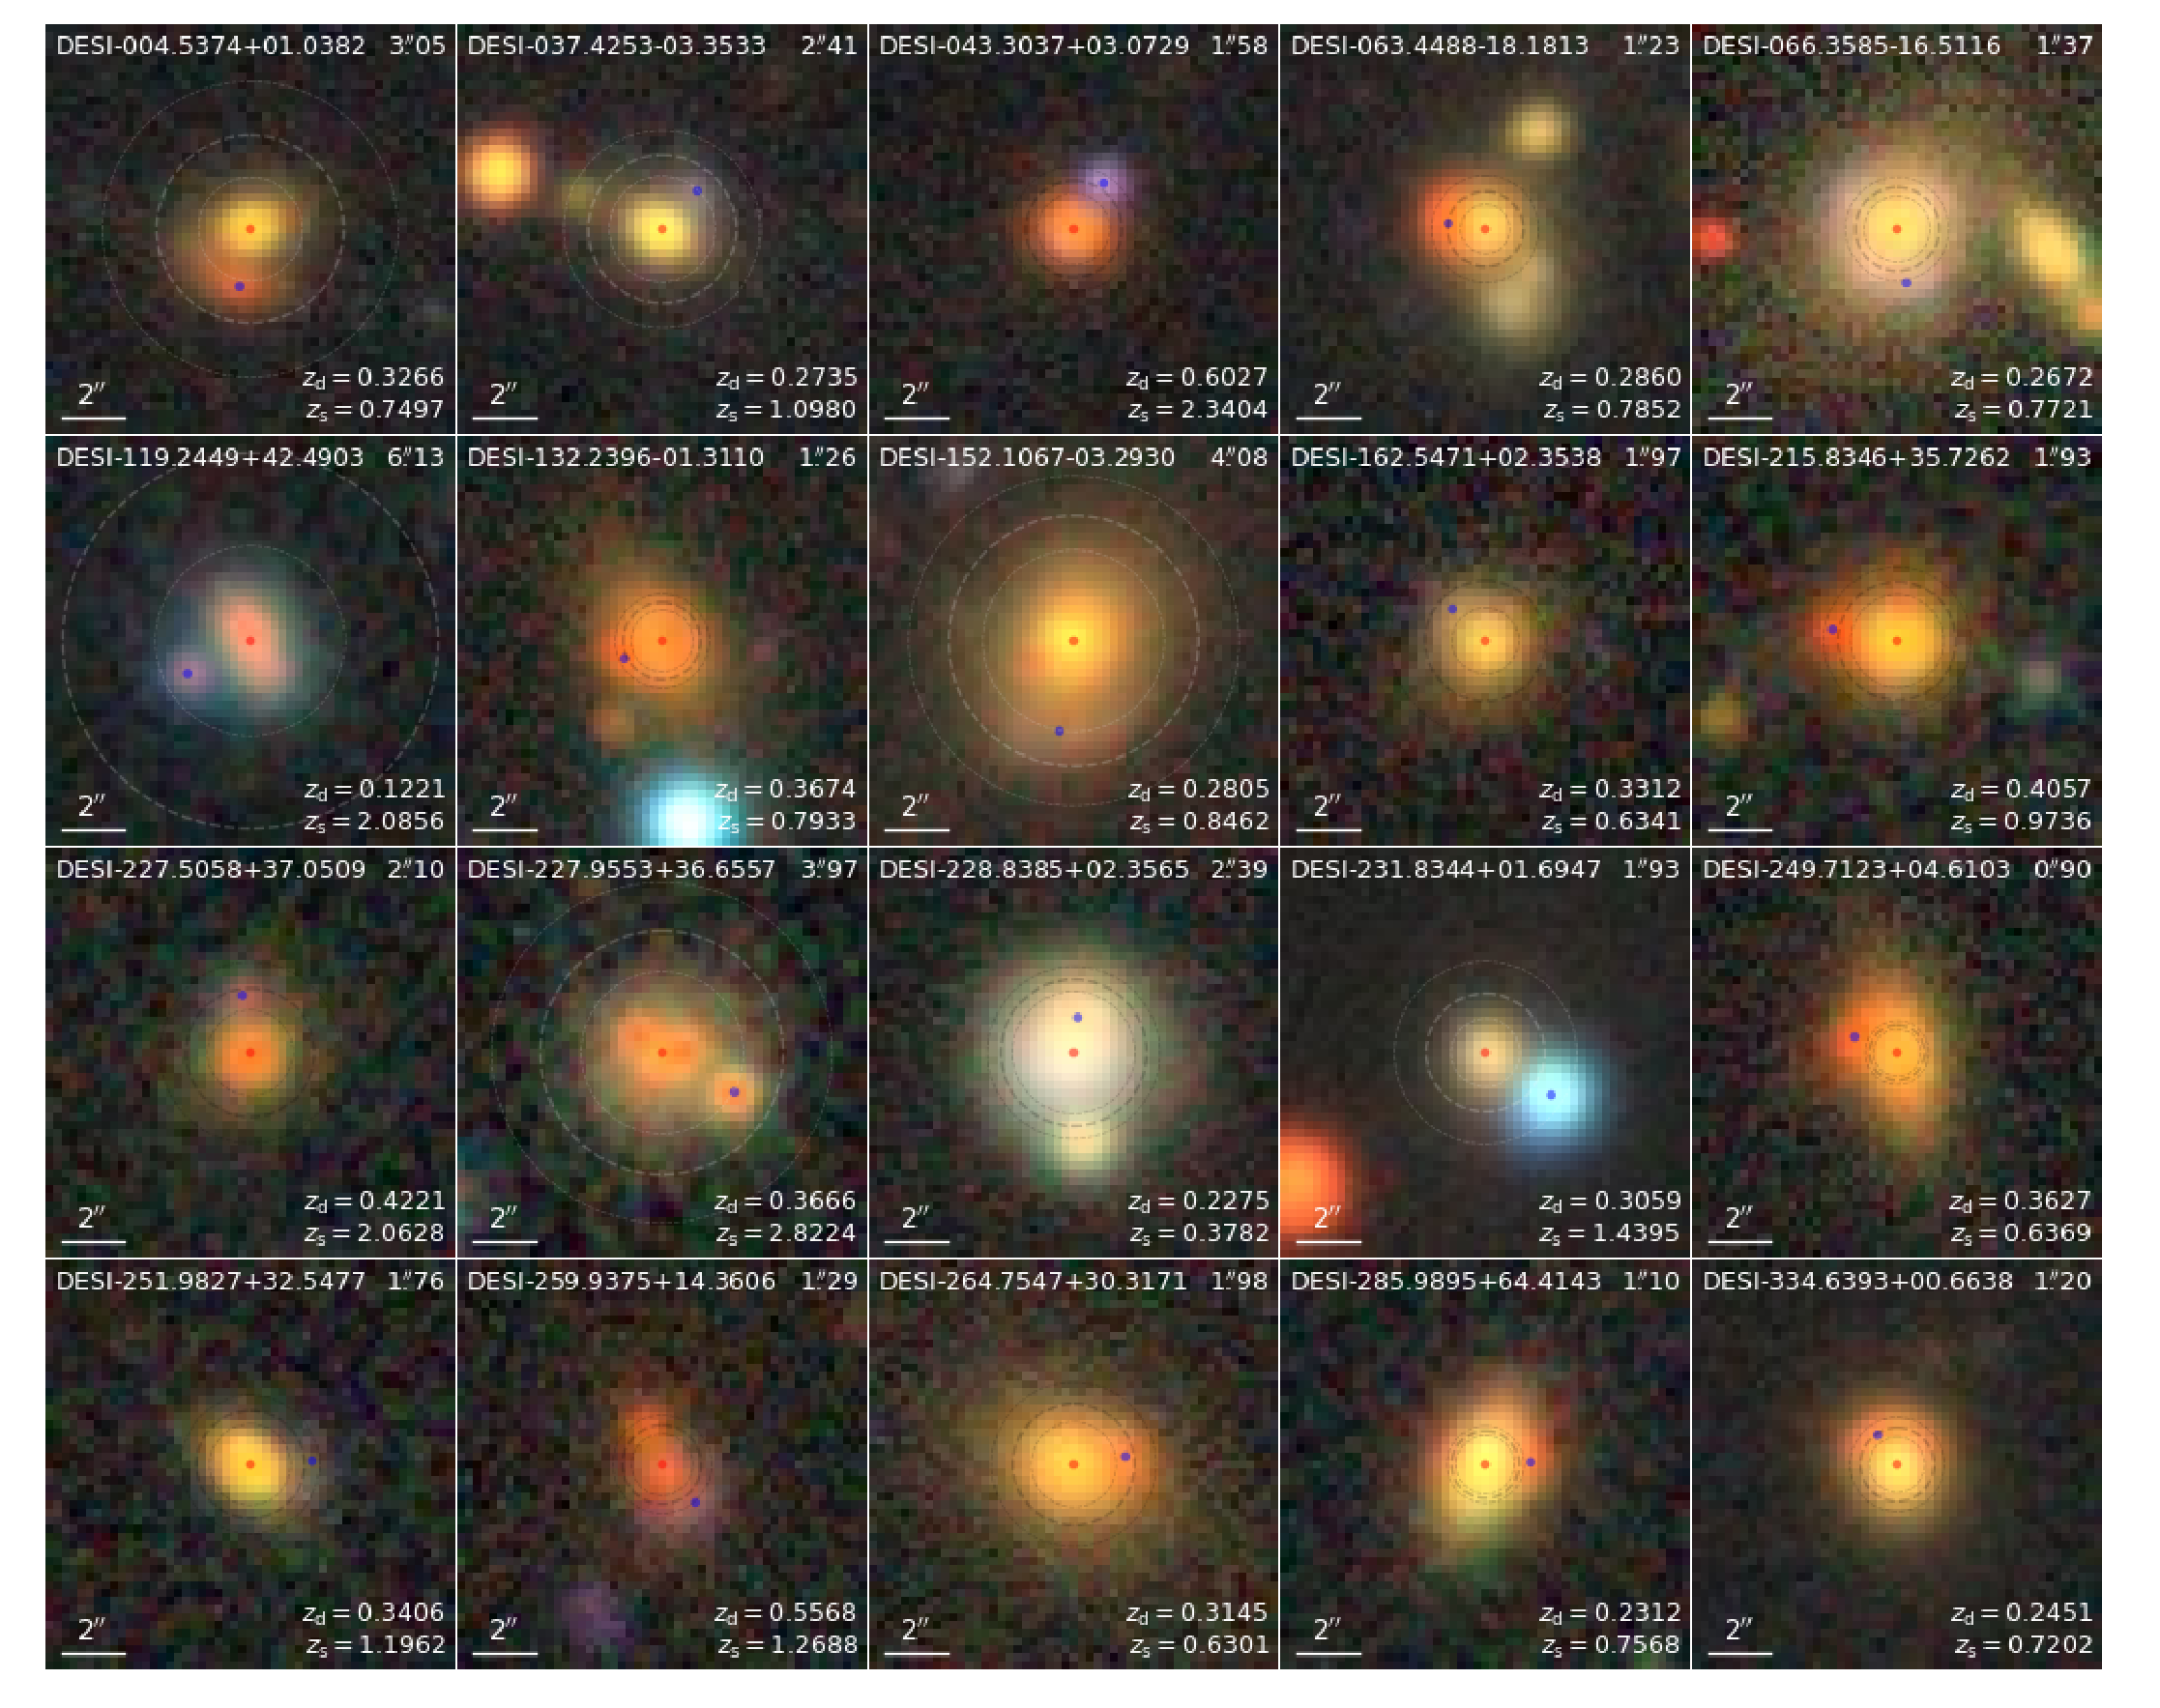
\includegraphics[width=\linewidth]{figures/orig_hsu-2025_fig3.png}\\[3pt]
  {\small\textbf{(b) \citet{hsu2025pairwise}, Fig.~3}}
\end{minipage}
\caption{\textbf{The 20 Grade A new lens candidates.} (a)~This work: DR10
$grz$ image cutouts at the centroids of the 20 \citet{hsu2025pairwise} Table~2
Grade A systems as recovered by our algorithmic pipeline, labelled with the
published name and the $(z_{\min}, z_{\max})$ redshift pair from our
$13{,}530$-group output (report Figure~\ref{fig:table2}). (b)~The published
Figure~3 showing the same 20 candidates, labelled with name and the
spectroscopic $(z_d, z_s)$ pair. All $20$ of $20$ are recovered within $3''$ of
our group centroids (median offset $0.91''$, maximum $1.54''$), with the matched
group redshifts reproducing the paper's $(z_d, z_s)$ columns to three decimal
places. Panel (b) reproduced from \citet{hsu2025pairwise}, their Fig.~3, for
comparison.}
\label{fig:cmp-hsu-2025-1}
\end{figure}

\bibliographystyle{plainnat}
\bibliography{references}

\end{document}
